\section{5. November 2012}
\setcounter{Aufg}{0} %Damit die Aufgaben jedes Mal bei Aufgabe 1 anfangen
\setcounter{Loes}{0}

\begin{Loes}
Es sei $\psi: (0, \infty) \times (0, 2\pi) \to \R^2 \setminus (\R_{\ge0} \times \{0\})$, $(r, \vartheta) \mapsto r(\cos \vartheta, \sin \vartheta)$, die Inverse $\varphi = \psi^{-1}$ ist eine Karte von $\R^2$.
\begin{align*}
	\pdifffrac[p]{}{r} &= \pdifffrac{\left(\Id^1 \circ \varphi^{-1}\right)}{r} \left(\varphi(p)\right) \pdifffrac[p]{}{x} + \pdifffrac{\left(\Id^2 \circ \varphi^{-1}\right)}{r} \left(\varphi(p)\right) \pdifffrac[p]{}{y}\\
	&= \pdifffrac{\left(\Id^1 \circ \psi\right)}{r} \left(\varphi(p)\right) \pdifffrac[p]{}{x} + \pdifffrac[p]{}{x} + \pdifffrac{\left(\Id^2 \circ \psi\right)}{r} \left(\varphi(r)\right)^2 \pdifffrac[p]{}{y}\\
	&= \cos\left(\vartheta(p)\right) \pdifffrac[p]{}{x} + \sin \left(\vartheta(p)\right) \pdifffrac[p]{}{y}\\
	&= \frac{1}{r(p)} \left(r(p) \cos\left(\vartheta(p)\right) \pdifffrac[p]{}{x} + r(p) \sin\left(\vartheta(p)\right) \pdifffrac[p]{}{y}\right)\\
	&= \frac{1}{r(p)} \left(\psi^1\left(\varphi(p)\right) \pdifffrac[p]{}{r} + \psi^2\left(\varphi(p)\right) \pdifffrac[p]{}{y}\right)\\
	&= \frac{1}{\|p\|} \left(p^1 \pdifffrac[p]{}{x} + p^2 \pdifffrac[p]{}{y}\right)
\end{align*}
Als Vektorfeld:
	\[ \pdifffrac{}{r} = \frac{1}{\|(x,y)\|} \left( x \pdifffrac{}{x} + y \pdifffrac{}{y} \right) \]
Desweiteren gilt:
\begin{align*}
	\pdifffrac[p]{}{\vartheta} &= \pdifffrac{\left(\Id^1 \circ \varphi^{-1}\right)}{\vartheta} \left( \varphi(p) \right) \pdifffrac[p]{}{x} + \pdifffrac{\left(\Id^2 \circ \varphi^{-1}\right)}{\vartheta} \left( \varphi(p) \right) \pdifffrac[p]{}{x}\\
	&= \ldots = -p_2\pdifffrac[p]{}{x} + p_1 \pdifffrac[p]{}{y}
\end{align*}
Also:
	\[ \pdifffrac{}{\vartheta} = -y \pdifffrac{}{x} + x \pdifffrac{}{y} \]
\begin{center}\begin{tikzpicture}
%\draw[step=0.25,gray!15] (-6,-3) grid (6,3); \draw[step=0.5,gray!30] (-6,-3) grid (6,3); \fill (0,0) circle(0.1); %Hilfsgitter
\draw[->] (-5,0) -- (-1,0); \draw[->] (1,0) -- (5,0); \draw[->] (-3,-2) -- (-3,2); \draw[->] (3,-2) -- (3,2);

\draw[->] (-1.5,0) -- (-1.5,1); \draw[->] (-3,1.5) -- (-4,1.5); \draw[->] (-4.5,0) -- (-4.5,-1); \draw[->] (-3,-1.5) -- (-2,-1.5);
\draw[->] (-1.875,0.875) -- ($(-1.875,0.875)+(-0.75,0.75)$); \draw[->] (-3.875, 1.125) --($(-3.875, 1.125)+(-0.75,-0.75)$);
\draw[->] (-4.125,-0.875) -- ($(-4.125,-0.875)+(0.75,-0.75)$); \draw[->] (-2.125, -1.125) -- ($(-2.125, -1.125)+(0.75,0.75)$);

\draw[->] (-2,0) -- (-2,0.5); \draw[->] (-3,1) -- (-3.5,1); \draw[->] (-4,0) -- (-4,-0.5); \draw[->] (-3,-1) -- (-2.5,-1);
\draw[->] (-2.25,0.5) -- ($(-2.25,0.5)+(-0.35,0.35)$); \draw[->] (-3.5,0.75) -- ($(-3.5,0.75)+(-0.35,-0.35)$);
\draw[->] (-3.75,-0.5) -- ($(-3.75,-0.5)+(0.35,-0.35)$); \draw[->] (-2.5,-0.75) -- ($(-2.5,-0.75)+(0.35,0.35)$);

\draw[->] (-2.5,0) -- (-2.5,0.25); \draw[->] (-3,0.5) -- (-3.25,0.5); \draw[->] (-3.5,0) -- (-3.5,-0.25); \draw[->] (-3,-0.5) -- (-2.75,-0.5);
\draw[->] (-2.625,0.25) -- ($(-2.625,0.25)+(-0.15,0.15)$); \draw[->] (-3.25,0.375) -- ($(-3.25,0.375)+(-0.15,-0.15)$);
\draw[->] (-3.375,-0.25) -- ($(-3.375,-0.25)+(0.15,-0.15)$); \draw[->] (-2.75,-0.375) -- ($(-2.75,-0.375)+(0.15,0.15)$);

\draw[->] (3.25,0.25) -- (3.75,0.75); \draw[->] (2.75,0.25) -- (2.25,0.75); \draw[->] (2.75,-0.25) -- (2.25,-0.75); \draw[->] (3.25,-0.25) -- (3.75,-0.75);
\draw[->] (2.75,0.75) -- (2.75,1.25); \draw[->] (2.25,0.25) -- (1.75,0.25);
\draw[->] (3.25,1) -- (3.5,1.5); \draw[->] (4.25,0.25) -- (4.75,0.5); \draw[->] (4,0.5) -- (4.5,0.875); \draw[->] (3.625,0.875) -- (4,1.375);
\draw[->] (3.625,1.625) -- (4.125,2.125); \draw[->] (4.25,1.5) -- (4.75,2); \draw[->] (4.75,1.25) -- (5.375,1.5);
\end{tikzpicture}\end{center}
\end{Loes}

\begin{Loes}\begin{enumerate}[label=\alph*),widest=b,leftmargin=*]
\item
	Zeige dass $\pi_i: M_1 \times M_2 \to M_i$, $(p_1,p_2) \mapsto p_i$ eine Submersion ist.
	
	Sei $(p_1,p_2) \in M_1 \times M_2$. Seien $\varphi_i$ Karten von $M_i$ um $p_i$ mit Kartengebieten $U_i$. Dann ist $\varphi_1 \times \varphi_2: U_1 \times U_2 \to \varphi_1(U_1) \times \varphi_2(U_2)$ eine Karte von $M_1 \times M_2$ um $(p_1,p_2)$. Es ist
		\[ \varphi_i \circ \pi_i \circ (\varphi_1 \times \varphi_2)^{-1} = \varphi_i \circ \pi_i \circ (\varphi_1^{-1} \times \varphi_2^{-1}). \]
	F"ur $(x_1,x_2) \in \varphi_1(U_1) \times \varphi_2(U_2)$ ist
		\[ \varphi_i \circ \pi_i \circ (\varphi_1 \times \varphi_2)^{-1} (x_1,x_2) = \varphi_i(\pi_i(\varphi_1^{-1}(x_1), \varphi_2^{-1}(x_2)))	= \varphi_i(\varphi_i^{-1}(x_i)) = x_i. \]
	Daraus folgt dass $\varphi_i \circ \pi_i \circ (\varphi_1 \times \varphi_2)^{-1}$ glatt ist. Der Rest des Beweises kann auf zwei Arten erfolgen.
	\begin{description}[font=\normalfont\itshape]
	\item[Variante 1:]
		Es folgt dass $\D(\varphi_i \circ \pi_i \circ (\varphi_1 \times \varphi_2)^{-1}) = \left( \begin{smallmatrix} 1 & & \\ & \ddots & \\ & & 1\\ & 0 &\end{smallmatrix} \right)$
		
		Dies ist die Darstellungsmatrix von $\pi_{1*}$ bez"uglich den Basen $\pdifffrac{}{\varphi_1^1}, \ldots, \pdifffrac{}{\varphi_1^d}$ und $\pdifffrac{}{(\varphi_1 \times \varphi_2)^1}, \ldots, \pdifffrac{}{(\varphi_1 \times \varphi_2)^{\ddim M_1 + \ddim M_2}}$. Also ist $\pi_{1*}$ surjektiv. Auch $\pi_1$ ist surjektiv, also ist $\pi_1$ eine Submersion. Der Beweis f"ur $\pi_2$ folgt analog.
	\item[Variante 2:]
		Sei $X = \sum_{j = 0}^{\ddim M_1} \xi^j \pdifffrac[p_1]{}{\varphi_1^j} \in \T_{p_1}M_1$. Setze
			\[ \tilde X = \sum_{j=1}^{\ddim M_1} \xi^j \pdifffrac[p]{}{(\varphi_1 \times \varphi_2)^j} \in \T_p(M_1 \times M_2). \]
		Dann ist
		\begin{align*}
			\pi_{1*_p} \tilde X &= \sum_{k=1}^{\ddim M_1} \left( \sum_j \underbrace{\partial_j \left( \varphi^k \circ \pi_1 \circ (\varphi_1 \times \varphi_2)^{-1} \right)}_{= \delta(k,j)} \left( \varphi_1(p_1), \varphi_2(p_2) \right) \xi^j \right) \pdifffrac[p_1]{}{\varphi_1^k}\\
			&= \sum_{k=1}^{\ddim M_1} \xi^k \pdifffrac[p_1]{}{\varphi_1^k} = X
		\end{align*}
		Daraus folgt dass $\pi_{1*}$ surjektiv ist.
	\end{description}
\item
	Zeige dass $f: (0,2\pi) \to \R^2$, $t \mapsto (\sin(t), \sin(2t))$ eine injektive Immersion aber keine Einbettung ist.
	\begin{description}[font=\normalfont\itshape]
	\item[$f$ ist injektiv:]
		Seien $t_1, t_2 \in (0,2\pi)$ mit $f(t_1) = f(t_2)$. Damit muss auch gelten dass $\sin(t_1) = \sin(t_2)$ und $\sin(2t_1) = \sin(2t_2)$. Aus diesen beiden Bedingungen folgt dass f"ur $t_1, t_2$ gelten muss:
		\begin{itemize}
		\item
			$t_1=t_2$ oder $\frac{\pi}{2}-t_1 = t_2-\frac{\pi}{2}$ oder $\frac{3\pi}{2}-t_1 = t_2 - \frac{3\pi}{2}$
		\item
			$2t_1=2t_2$ oder $\frac{\pi}{2}-2t_1=2t_2-\frac{\pi}{2}$ oder $\frac{3\pi}{2}-2t_1=2t_2-\frac{3\pi}{2}$
		\end{itemize}
		Aus den beiden Bedingungen folgt somit dass $t_1 = t_2$ gilt.
	\item[$f$ ist eine Immersion:]
		Es reicht zu zeigen, dass $f_{*t} = 0$ f"ur alle $t$ gilt. Es gilt $\D f(t) = (\cos(t), 2 \cos(2t))$, also
		\begin{align*}
			\D f(t) = 0 & \Leftrightarrow \cos(t) = 0 \text{ und } \cos(2t)=0\\
			& \Leftrightarrow \left(t = \frac{\pi}{2} \vee t = \frac{3\pi}{2} \right) \bigwedge \left( 2t = \frac{\pi}{2} \vee 2t = \frac{3\pi}{2} \vee 2t = \frac{5\pi}{2} \vee 2t = \frac{7\pi}{2}\right)
		\end{align*}
		Das ist aber nicht m"oglich, also ist $\D f(t) \ne 0$. $\D f(t)$ ist die Darstellungsmatrix, also ist auch $f_{*_t} \ne 0$.
	\item[$f$ ist keine Einbettung:]
		\marginnote{\emph{Skizze:}\\
			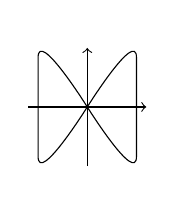
\begin{tikzpicture}[scale=0.25,baseline=0]
				%\draw[step=0.25,gray!15] (-6,-3) grid (6,3); \draw[step=0.5,gray!30] (-6,-3) grid (6,3); \fill (0,0) circle(0.1); %Hilfsgitter
				\draw[->] (-3,0) -- (3,0); \draw[->] (0,-3) -- (0,3);
				\def\streck{4}		
				\draw (0,0) ..controls(0,0) and (2.5,\streck).. (2.5,2.5) -- (2.5,-2.5) ..controls(2.5,-\streck) and (0,0).. (0,0) ..controls(0,0) and (-2.5,\streck)..  (-2.5,2.5) -- (-2.5,-2.5) ..controls(-2.5,-\streck) and (0,0).. (0,0) -- cycle;
			\end{tikzpicture}}
		Es gilt dass $\left( \frac{1}{k} \right)_{k \in \N}$ nicht in $(0,2\pi)$ konvergiert, aber es ist $f\left( \frac{1}{k} \right) \to (0,0) = f(\pi) \in \Bild f$. Damit ist $f$ kein Hom"oomorphismus auf das Bild.
	\end{description}
\end{enumerate}\end{Loes}

\setcounter{Loes}{3}
\begin{Loes}
Zeige dass die Gruppen $\SL(n,\R) = \{A \in \R^{n\times n} | \ddet A = 1\}$ und $\Oo(n,\R) = \{A \in \R^{n \times n} | AA^T = I_n\}$ glatte Untermannigfaltigkeiten des $R^{n \times n}$ sind.

Definiere $f = \det$, dann ist $\SL(n, \R) = f^{-1}(1)$. Dann gilt\marginnote{\scriptsize{\textcolor{gray}{$A[k,j]$ bezeichnet die Matrix $A$ bei der die $k$-te Zeile und die $i$-te Spalte weggelassen wurden}}}
	\[\pdifffrac{(f)}{a_{ij}} = \pdifffrac{}{a_{ij}} \left( \sum_{k=1}^n(-1)^{k+j} \ddet A[k,j]a_{jk} \right) = (-1)^{i+j} \ddet A[i,j]\]
Es ist $\D f(A) = 0 \Leftrightarrow \forall i,j \ddet A[i,j] = 0 \Rightarrow \ddet A = 0$, damit ist $1$ regul"arer Wert. Also ist $\ddim \SL(n,\R) = \ddim \R^{n\times n} - \ddim \R = n^2 -1$.

Definiere nun $g: \R^{n \times n} \to \R^{n \X n}$, $A \mapsto AA^T$. Dann ist $\Oo(n) = g^{-1}(I_n)$ und es gilt
	\begin{align*}
		\D g(A)(B) &= \difffrac[t=0]{}{t} g(A + tB)\\
		&= \difffrac[t=0]{}{t} (AA^T + tAB^T + tBA + t^2BB^T) = AB^T + BA^T
	\end{align*}
	Seien nun $A \in \Oo(n,\R)$ und $C \in \R_{\text{sym}}^{n \X n}$. Es bleibt zu zeigen dass ein $B \in \R^{n \X n}$ existiert sodass $\D g(A)(B) = C$. Es gilt:
		\[ \D g\left(A\right)\left(\frac{1}{2}CA\right) = \frac{1}{2} \left( \underbrace{AA^T}_{=I}C^T + C\underbrace{AA^T}_{=I} \right) = C \]
	Daraus folgt dass $I$ ein regul"arer Wert von $g$ ist und $\Oo(n,\R)$ eine Untermannigfaltigkeit von $\R^{n \X n}$ der Dimension $n^2-\ddim \R_{\text{sym}}^{n \X n} = n^2 - \frac{n(n+1)}{2} = \frac{n(n-1)}{2}$.
\end{Loes}